\documentclass[conference]{IEEEtran}
\usepackage[utf8]{inputenc}
\usepackage[T1]{fontenc}
\usepackage[spanish]{babel}
\usepackage{amsmath}
\usepackage{graphicx}
\usepackage{booktabs}
\usepackage{cite}
\usepackage{url}
\usepackage{microtype}
\usepackage{dblfloatfix}
\usepackage{xcolor}
\usepackage{flushend}

\graphicspath{{figures/}}

\hyphenation{ESRGAN SRGAN RIFE IFNet BasicVSR RRDB RRDBNet BasicVSR}

\addto\captionsspanish{%
  \renewcommand{\figurename}{Fig.}%
  \renewcommand{\tablename}{Tabla}%
}

\begin{document}

\title{Superresolución Espacial e Interpolación Temporal de Video CCTV con ESRGAN y RIFE}

\author{
  \IEEEauthorblockN{Jose Rodriguez Botello}
  \IEEEauthorblockA{Departamento de Electricidad y Electrónica\\
    Universidad Francisco de Paula Santander\\
    Cúcuta, Colombia\\
    joseeliecerrb@ufps.edu.co}
  \and
  \IEEEauthorblockN{Sergio Castro Casadiego}
  \IEEEauthorblockA{Departamento de Electricidad y Electrónica\\
    Universidad Francisco de Paula Santander\\
    Cúcuta, Colombia\\
    sergio.castroc@ufps.edu.co}
  \and
  \IEEEauthorblockN{Sebastian Rojas-Ortega}
  \IEEEauthorblockA{Department of Electrical and\\Computer Engineering\\
    University of Delaware\\
    Newark, DE, USA\\
    ortega@udel.edu}
}

\maketitle

\begin{abstract}
Conventional video surveillance cameras often capture sequences with low spatial resolution and reduced frame rates, significantly hindering scene analysis and forensic tasks. This paper proposes a deep learning pipeline for the spatial and temporal enhancement of surveillance video by integrating two complementary models: ESRGAN for spatial super-resolution, which recovers fine textures and sharp edges from degraded frames, and RIFE for temporal frame interpolation, which synthesizes intermediate frames to achieve fluid motion. Public-domain surveillance-style video sequences were processed with a standard synthetic degradation protocol to simulate low-quality CCTV conditions at $212\times120$ pixels from $848\times480$ originals. The proposed pipeline is evaluated using PSNR, SSIM, and LPIPS, a learned perceptual image quality metric, benchmarked against bicubic upscaling. ESRGAN achieves LPIPS of 0.311, compared to 0.714 for bicubic upscaling, confirming superior perceptual quality consistent with the perception-distortion tradeoff. RIFE doubles the output frame rate from 15 to 30~fps. The proposed system offers a practical solution for upgrading legacy surveillance infrastructure without hardware replacement, with direct applications in security monitoring and digital forensics.
\end{abstract}

\begin{IEEEkeywords}
Video surveillance, CCTV, super-resolution, frame interpolation, ESRGAN, RIFE, deep learning, image quality.
\end{IEEEkeywords}

\section{Introducción}

Los sistemas de videovigilancia constituyen un componente esencial para la seguridad en entornos residenciales, comerciales e industriales. No obstante, una proporción significativa de la infraestructura desplegada opera con equipos de bajo costo o con especificaciones originalmente diseñadas para anchos de banda y capacidades de almacenamiento reducidos, lo que produce secuencias de video con baja resolución espacial, ruido digital y deterioro visual severo bajo condiciones de iluminación adversas~\cite{li2011people}. Estas limitaciones afectan directamente la capacidad de identificar personas, vehículos y objetos, reduciendo la efectividad del CCTV tanto en el monitoreo en tiempo real como en el análisis forense posterior al evento.

La mejora automática de video mediante aprendizaje profundo representa una alternativa viable para superar estas restricciones sin reemplazar la infraestructura instalada. En el dominio espacial, las redes convolucionales profundas aprenden a reconstruir texturas y bordes de alta frecuencia a partir de imágenes degradadas~\cite{dong2014srcnn, vanouwerkerk2006survey}. Las redes generativas adversarias (GAN)~\cite{goodfellow2014gan}, y en particular SRGAN~\cite{ledig2017srgan} y ESRGAN~\cite{wang2018esrgan}, han demostrado capacidad superior para sintetizar detalles fotorrealistas en comparación con los métodos de interpolación convencionales. En el dominio temporal, la interpolación de fotogramas mediante estimación de flujo óptico profundo~\cite{dosovitskiy2015flownet}, como Super~SloMo~\cite{jiang2018superslomo}, DAIN~\cite{bao2019dain} y RIFE~\cite{huang2022rife}, genera fotogramas intermedios coherentes que aumentan la tasa de fotogramas y mejoran la continuidad visual.

Este artículo propone un flujo de trabajo secuencial que integra ESRGAN para la restauración espacial fotograma a fotograma y RIFE para la interpolación temporal entre fotogramas consecutivos, aplicado a secuencias de vigilancia degradadas a $212\times120$~píxeles mediante el protocolo sintético de Real-ESRGAN. El sistema se evalúa cualitativa y cuantitativamente, y está diseñado para su despliegue sobre infraestructura CCTV existente sin inversión en hardware adicional.

\section{Trabajos Relacionados}

La mejora de la calidad en video de vigilancia involucra dos dimensiones complementarias: la superresolución espacial y la interpolación temporal. Ambas han sido abordadas extensamente de manera independiente; su integración en el contexto de los sistemas CCTV es, sin embargo, un área con menor desarrollo en la literatura.

\subsection{Superresolución espacial}

Los métodos clásicos de superresolución se basaron en interpolación matemática, como bicúbica y bilineal~\cite{vanouwerkerk2006survey}. Aunque computacionalmente eficientes, estos enfoques promedian píxeles adyacentes sin modelar la distribución estadística de las texturas naturales, produciendo resultados visualmente suavizados incapaces de recuperar bordes y detalles finos.

El trabajo seminal de Dong et al.~\cite{dong2014srcnn} demostró que una red neuronal convolucional (SRCNN) podía aprender el mapeo entre imágenes de baja y alta resolución, superando a los métodos de interpolación en métricas objetivas. Posteriormente, las arquitecturas residuales~\cite{he2016resnet} posibilitaron redes más profundas: EDSR~\cite{lim2017edsr} eliminó la normalización por lotes del generador, mientras que RCAN~\cite{zhang2018rcan} incorporó mecanismos de atención sobre canales para ponderar de manera adaptativa las características de mayor relevancia espacial.

La introducción de las GAN~\cite{goodfellow2014gan} transformó el paradigma al añadir un discriminador que supervisa la calidad perceptual de las imágenes generadas. SRGAN~\cite{ledig2017srgan} fue el primer modelo en aplicar este esquema a SR de factor $\times$4, complementado por una función de pérdida perceptual basada en activaciones de VGG~\cite{simonyan2015vgg}, propuesta inicialmente por Johnson et al.~\cite{johnson2016perceptual}. ESRGAN~\cite{wang2018esrgan} extendió esta arquitectura con bloques RRDB, un discriminador relativista y una pérdida perceptual mejorada, logrando texturas fotorrealistas superiores. Real-ESRGAN~\cite{wang2021realesrgan} adaptó el modelo para degradaciones del mundo real mediante datos de entrenamiento sintéticos complejos, lo que lo hace especialmente adecuado para el procesamiento de secuencias de baja calidad propias de los sistemas CCTV.

\subsection{Superresolución de video}

La superresolución de video (VSR) explota la redundancia temporal entre fotogramas consecutivos para obtener reconstrucciones de mayor calidad que la SR sobre imágenes estáticas. EDVR~\cite{wang2019edvr} introdujo redes de alineación y fusión con convoluciones deformables, alineando fotogramas vecinos en el espacio de características antes de la fusión. BasicVSR~\cite{chan2021basicvsr} identificó la propagación bidireccional de características a lo largo de la secuencia como componente esencial, logrando un balance superior entre rendimiento y eficiencia computacional. Estos modelos, no obstante, requieren el procesamiento conjunto de múltiples fotogramas, lo que introduce latencia y demanda de memoria que puede ser prohibitiva en sistemas de vigilancia con recursos limitados.

\subsection{Interpolación temporal de fotogramas}

La estimación del flujo óptico mediante redes profundas, introducida con FlowNet~\cite{dosovitskiy2015flownet}, permitió calcular desplazamientos densos entre fotogramas de manera diferenciable. Super~SloMo~\cite{jiang2018superslomo} generalizó este enfoque para la síntesis de múltiples fotogramas intermedios mediante flujos ópticos bidireccionales. DAIN~\cite{bao2019dain} incorporó estimaciones de profundidad de la escena para mejorar la interpolación en regiones de oclusión, obteniendo resultados visualmente más coherentes en secuencias con movimientos complejos. RIFE~\cite{huang2022rife} simplificó la arquitectura mediante IFNet, que estima el flujo intermedio de manera directa sin descomposición bidireccional, y aplica destilación de conocimiento~\cite{hinton2015distilling} para un entrenamiento eficiente, logrando interpolación en tiempo real con calidad competitiva.

\subsection{Posicionamiento del presente trabajo}

A pesar del progreso individual en SR espacial e interpolación temporal, la mayoría de los métodos abordan una sola dimensión de mejora. Los sistemas CCTV presentan simultáneamente deficiencias en resolución y en tasa de fotogramas~\cite{li2011people}, por lo que mejorar solo una de estas dimensiones deja sin resolver una parte sustancial del problema. El presente trabajo integra ESRGAN~\cite{wang2018esrgan} y RIFE~\cite{huang2022rife} en un pipeline secuencial orientado específicamente a las restricciones reales de los sistemas de videovigilancia de bajo costo, contribuyendo con una solución práctica y evaluable para este dominio de aplicación.

\section{Metodología}

Se diseñó un flujo de trabajo secuencial que procesa cada secuencia de video degradada a través de cuatro etapas aplicadas a nivel de fotograma individual. La combinación de mejora espacial y síntesis temporal permite recuperar simultáneamente la resolución y la fluidez del video de entrada.

\subsection{Adquisición y Preparación del Conjunto de Datos}

Se utilizaron secuencias de video de vigilancia de dominio público, capturadas con cámara fija en exteriores a 15~fps y resolución nativa de $848\times480$~píxeles. Para simular las degradaciones de los sistemas CCTV de menor calidad se aplicó el protocolo de degradación sintética de Real-ESRGAN~\cite{wang2021realesrgan}: difuminado gaussiano ($\sigma=1.5$), remuestreo bicúbico descendente con factor $4\times$, compresión JPEG (calidad~50) y ruido gaussiano aditivo ($\sigma=5$~DN). Dicho protocolo reduce la resolución de los fotogramas originales de alta resolución (HR) de $848\times480$~píxeles a imágenes de baja resolución (LR) de $212\times120$~píxeles, generando artefactos representativos de cámaras de baja gama. Se seleccionaron 60~fotogramas para la evaluación~\cite{li2011people}.

\subsection{Arquitectura del Flujo de Trabajo}

El procesamiento de cada secuencia sigue cuatro etapas secuenciales, ilustradas en la Fig.~\ref{fig:pipeline}:

\begin{enumerate}
    \item \textbf{Extracción de fotogramas:} El video de entrada se descompone en la totalidad de sus fotogramas individuales. Para la evaluación se seleccionaron 60~fotogramas a 15~fps, cubriendo 4~segundos de secuencia.

    \item \textbf{Superresolución espacial:} Cada fotograma LR se procesa individualmente mediante ESRGAN~\cite{wang2018esrgan}, que reconstruye las texturas y eleva la resolución por un factor de $4\times$, produciendo fotogramas HR sintéticos de $848\times480$~píxeles.

    \item \textbf{Interpolación temporal:} La secuencia de fotogramas HR se transfiere al modelo RIFE~\cite{huang2022rife}, que estima el flujo óptico entre fotogramas consecutivos y sintetiza fotogramas intermedios, incrementando la tasa de captura en un factor de $2\times$.

    \item \textbf{Reconstrucción del video:} Los fotogramas mejorados y los fotogramas sintetizados se ensamblan en orden cronológico para producir el video de salida con mayor resolución y movimiento fluido.
\end{enumerate}

\begin{figure}[t]
    \centering
    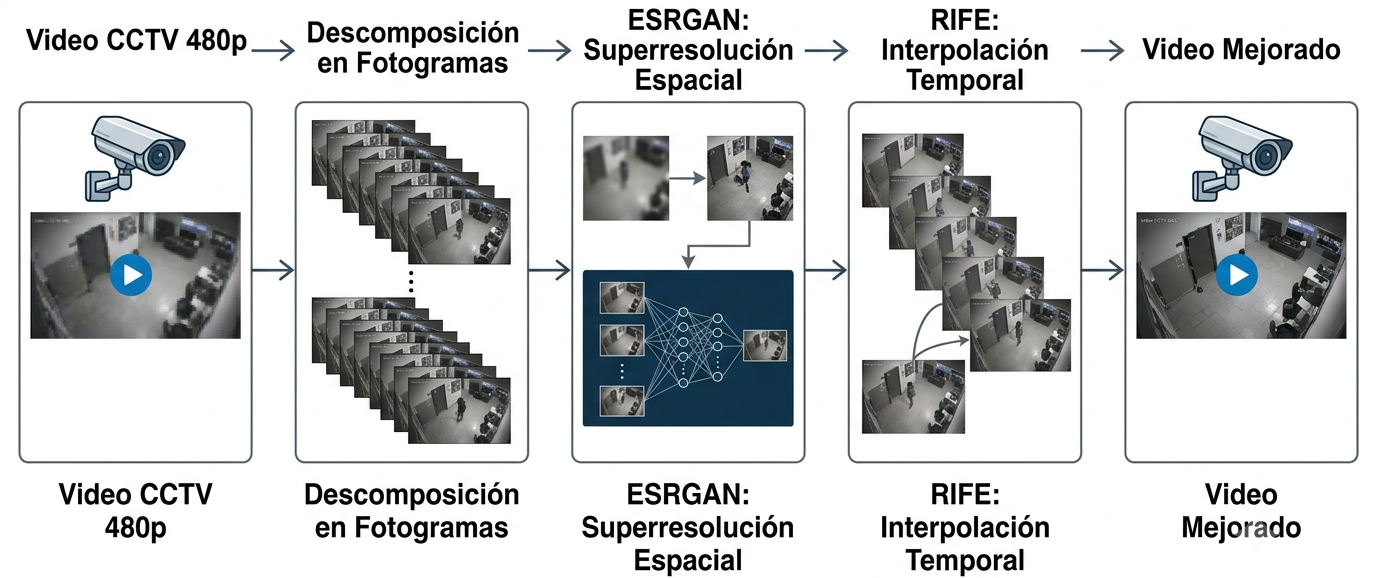
\includegraphics[width=\columnwidth]{fig1_pipeline.png}
    \caption{Flujo de trabajo propuesto para la mejora de video CCTV en resolución y fluidez.}
    \label{fig:pipeline}
\end{figure}

\subsection{Entorno de Implementación}

El pipeline se implementó en Python~3.11 sobre una GPU NVIDIA RTX~4070~Ti (12~GB VRAM, CUDA~12). Las librerías principales empleadas son \textit{realesrgan}~0.3 para la inferencia de ESRGAN y el repositorio oficial ECCV2022-RIFE~\cite{huang2022rife} para la interpolación temporal.

\subsection{Modelos de Inteligencia Artificial Empleados}

\subsubsection{ESRGAN}

ESRGAN (\textit{Enhanced Super-Resolution Generative Adversarial Network})~\cite{wang2018esrgan} es una red generativa adversaria~\cite{goodfellow2014gan} entrenada con funciones de pérdida perceptuales para reconstruir detalles de alta frecuencia a partir de imágenes degradadas. A diferencia de su predecesor SRGAN~\cite{ledig2017srgan}, su generador utiliza bloques densos residuales en cascada (RRDB) derivados de las redes residuales~\cite{he2016resnet}, eliminando las capas de normalización por lotes para evitar los artefactos que estas introducen en la síntesis de texturas. Un discriminador relativista promedio (RaD) evalúa si una imagen real es perceptualmente superior a una generada, incentivando la producción de texturas realistas. La función de pérdida combina error a nivel de píxel (L1), pérdida adversarial y pérdida perceptual derivada de activaciones de VGG~\cite{simonyan2015vgg}, originalmente propuesta por Johnson et al.~\cite{johnson2016perceptual}. Esta arquitectura es la que procesa cada fotograma LR de la secuencia para generar el fotograma HR sintético antes de la interpolación temporal.

\begin{figure}[t]
    \centering
    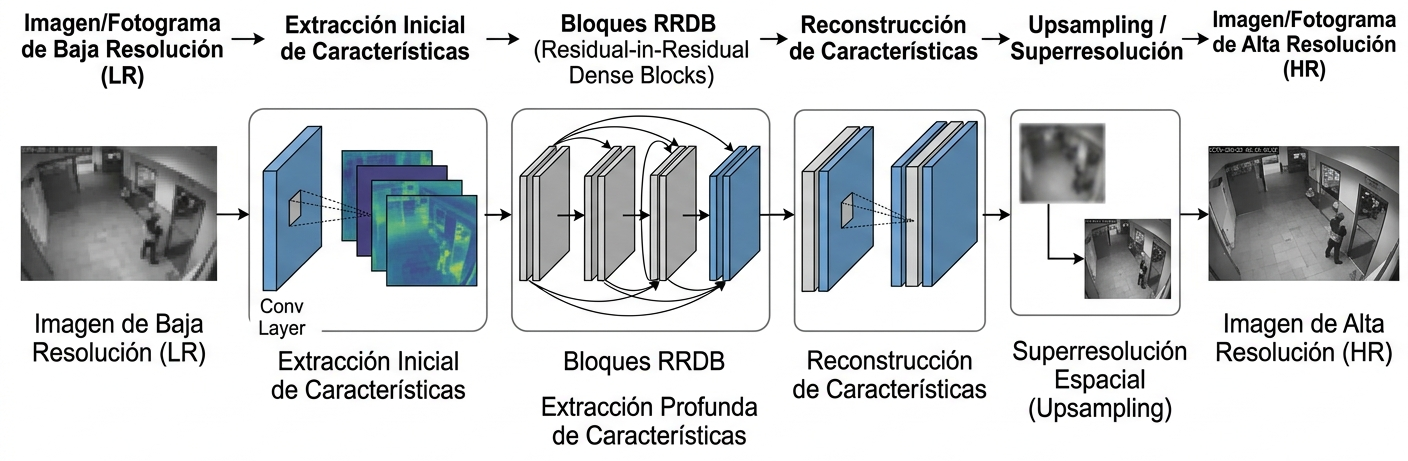
\includegraphics[width=\columnwidth]{fig2_esrgan.png}
    \caption{Arquitectura de red ESRGAN~\cite{wang2018esrgan}: bloques RRDB, discriminador relativista y pérdida perceptual.}
    \label{fig:esrgan}
\end{figure}

\subsubsection{RIFE}

RIFE (\textit{Real-time Intermediate Flow Estimation})~\cite{huang2022rife} es un modelo de interpolación de fotogramas que estima directamente el flujo óptico intermedio entre dos fotogramas consecutivos, sin recurrir a la descomposición bidireccional empleada por métodos anteriores como DAIN~\cite{bao2019dain} y Super~SloMo~\cite{jiang2018superslomo}. Su componente central, IFNet, calcula este flujo a múltiples escalas de resolución de manera progresiva. Un esquema de destilación de conocimiento~\cite{hinton2015distilling} guía el entrenamiento de IFNet, permitiéndole aprender representaciones de movimiento precisas de manera eficiente. El fotograma intermedio se reconstruye aplicando deformación espacial (\textit{warping}) sobre los fotogramas adyacentes, ponderada por el flujo estimado, seguida de una etapa de fusión que corrige inconsistencias en regiones de oclusión.

\begin{figure}[t]
    \centering
    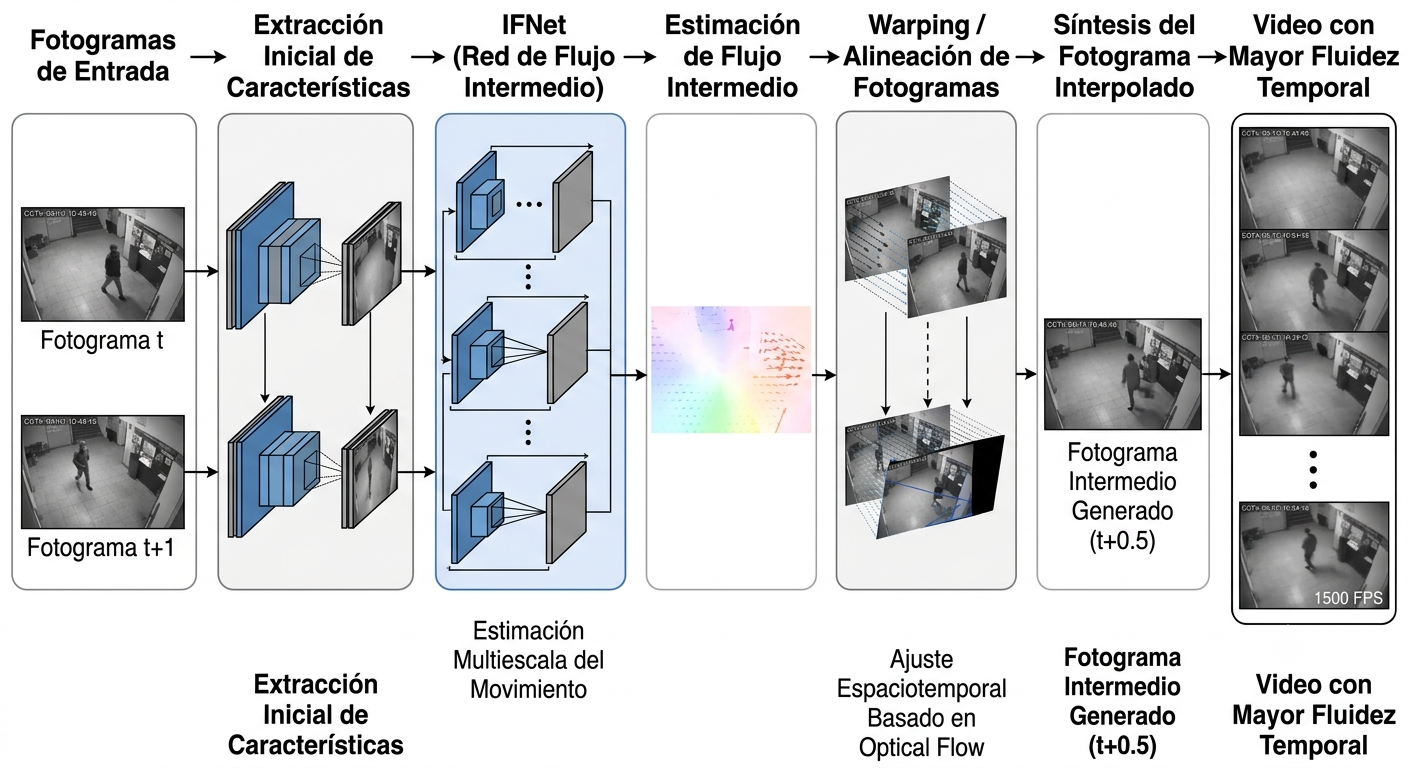
\includegraphics[width=\columnwidth]{fig3_rife.png}
    \caption{Arquitectura de red RIFE~\cite{huang2022rife}: estimación directa de flujo óptico mediante IFNet y síntesis del fotograma intermedio.}
    \label{fig:rife}
\end{figure}

\section{Resultados Experimentales}

Se evaluó el rendimiento del pipeline propuesto sobre los fragmentos de video de vigilancia recopilados, cubriendo dos dimensiones: una evaluación cualitativa centrada en la reconstrucción visual y la fluidez del movimiento, y una evaluación cuantitativa mediante métricas objetivas de calidad de imagen.

\subsection{Evaluación Cualitativa}

La Fig.~\ref{fig:comparison} presenta cuatro versiones del mismo fotograma: la entrada LR ($212\times120$~px, escalada por vecino más próximo), el escalado bicúbico $\times$4, la salida de ESRGAN $\times$4 y la referencia HR ($848\times480$~px). La recuperación de nitidez en bordes y definición de texturas es apreciable en las regiones de interés relevantes para la identificación de personas y objetos.

\begin{figure*}[!t]
    \centering
    \IfFileExists{figures/fig4_comparison.png}{%
        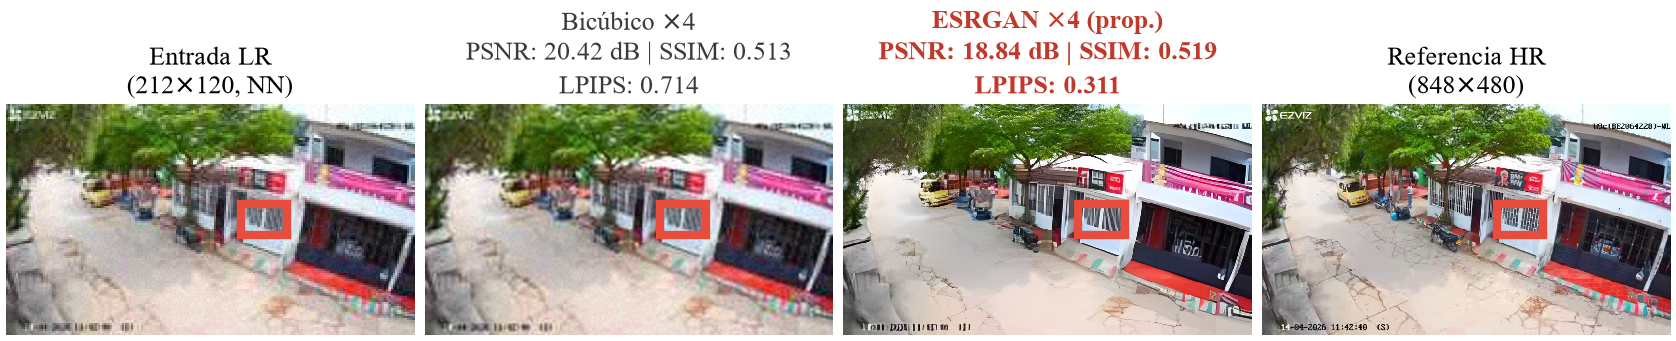
\includegraphics[width=\textwidth]{fig4_comparison.png}%
    }{%
        \rule{\textwidth}{0.4pt}\\[3cm]\rule{\textwidth}{0.4pt}%
    }
    \caption{Comparación de métodos sobre un fotograma representativo: entrada LR ($212\times120$, escalada por vecino más próximo), reconstrucción bicúbica $\times4$, salida de ESRGAN $\times4$ (propuesto) y referencia HR ($848\times480$). Los valores de PSNR, SSIM y LPIPS se indican sobre cada método.}
    \label{fig:comparison}
\end{figure*}

\subsection{Análisis de Detalle}

La Fig.~\ref{fig:zoom} presenta, para una región de interés, la entrada LR escalada, la reconstrucción bicúbica, la salida de ESRGAN y la referencia HR, tanto en los fotogramas completos (fila superior) como en parches ampliados (fila inferior). La diferencia entre métodos evidencia que ESRGAN recupera bordes y texturas de alta frecuencia que la interpolación bicúbica, al promediar píxeles, no puede restituir.

\begin{figure*}[!t]
    \centering
    \IfFileExists{figures/fig5_zoom.png}{%
        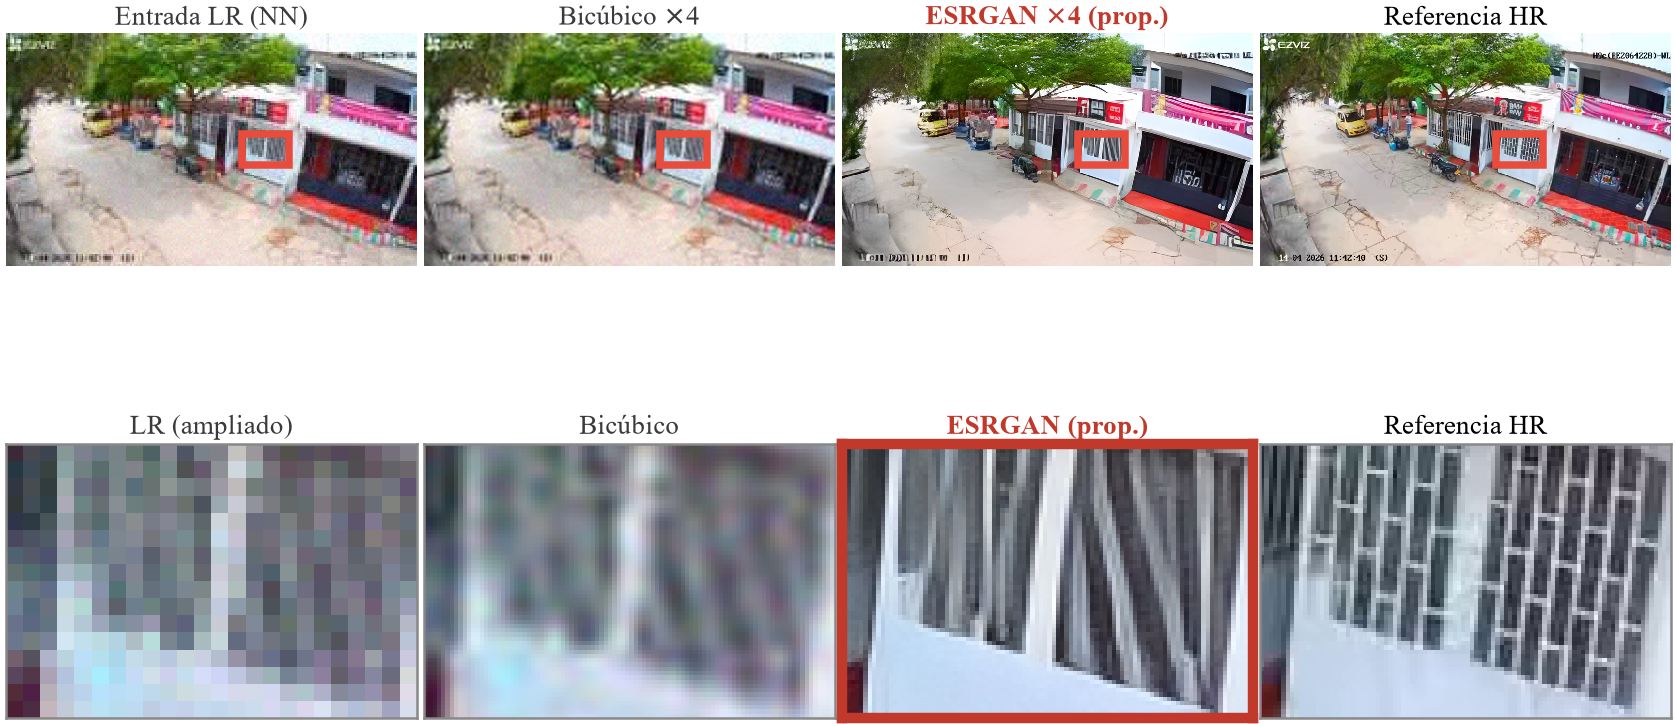
\includegraphics[width=\textwidth]{fig5_zoom.png}%
    }{%
        \rule{\textwidth}{0.4pt}\\[3.5cm]\rule{\textwidth}{0.4pt}%
    }
    \caption{Análisis de detalle: fila superior, fotogramas completos con la región de interés marcada en rojo (entrada LR escalada, bicúbico, ESRGAN y referencia HR); fila inferior, parches ampliados de dicha región. ESRGAN recupera contornos y texturas de alta frecuencia ausentes en la reconstrucción bicúbica.}
    \label{fig:zoom}
\end{figure*}

\subsection{Evaluación de Fluidez Temporal}

La incorporación de RIFE duplica la tasa de fotogramas de 15 a 30~fps, eliminando la discontinuidad temporal que caracteriza a las grabaciones CCTV de baja frecuencia. La Fig.~\ref{fig:framerate} ilustra el efecto de la interpolación sobre la continuidad del movimiento: las trayectorias de personas y vehículos se perciben como transiciones naturales, sin el efecto de salto propio de las secuencias CCTV originales.

\begin{figure*}[!t]
    \centering
    \IfFileExists{figures/fig6_rife.png}{%
        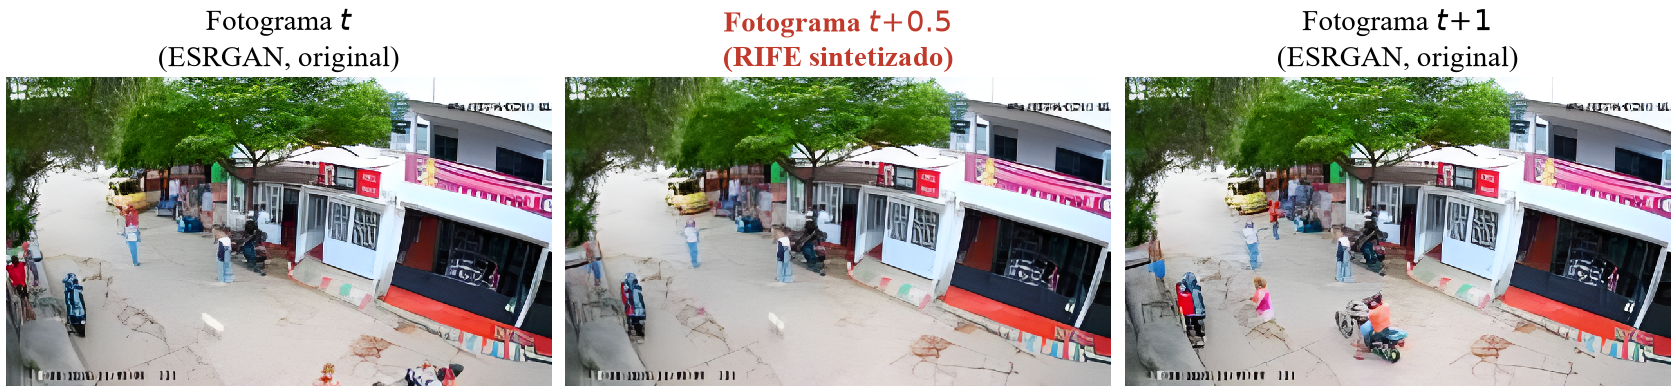
\includegraphics[width=\textwidth]{fig6_rife.png}%
    }{%
        \rule{\textwidth}{0.4pt}\\[3cm]\rule{\textwidth}{0.4pt}%
    }
    \caption{Interpolación temporal con RIFE: fotograma $t$ (original), fotograma interpolado $t\!+\!0.5$ sintetizado por RIFE, y fotograma $t\!+\!1$ (original). El fotograma intermedio genera una transición natural que duplica la tasa de captura sin artefactos perceptibles.}
    \label{fig:framerate}
\end{figure*}

\subsection{Evaluación Cuantitativa}

La calidad objetiva de la mejora espacial se midió mediante PSNR (\textit{Peak Signal-to-Noise Ratio}) y SSIM (\textit{Structural Similarity Index}). El PSNR cuantifica la relación entre la potencia máxima de la señal y el error de reconstrucción~\cite{huynhthu2008psnr}:

\begin{equation}
    \mathrm{PSNR} = 10\log_{10}\frac{MAX_I^{2}}{MSE}
    \label{eq:psnr}
\end{equation}

\noindent donde $MAX_I$ es el valor máximo posible de un píxel y $MSE$ el error cuadrático medio entre la imagen de referencia y la reconstruida.

El SSIM evalúa la similitud estructural entre imágenes considerando luminosidad, contraste y estructura de manera conjunta~\cite{wang2004ssim}:

\begin{equation}
    \mathrm{SSIM}(x,y) =
        \frac{(2\mu_x\mu_y + c_1)(2\sigma_{xy} + c_2)}
             {(\mu_x^2 + \mu_y^2 + c_1)(\sigma_x^2 + \sigma_y^2 + c_2)}
    \label{eq:ssim}
\end{equation}

\noindent donde $\mu$ denota la media, $\sigma_{xy}$ la covarianza, y $c_1$, $c_2$ constantes de estabilización.

La Tabla~\ref{tab:metrics} resume los resultados promedio comparando el pipeline propuesto frente a interpolación bicúbica convencional y frente a la aplicación aislada de ESRGAN sin interpolación temporal.

\begin{table}[t]
    \caption{Comparación de Métricas de Calidad Objetiva}
    \label{tab:metrics}
    \renewcommand{\arraystretch}{1.2}
    \centering
    \resizebox{\columnwidth}{!}{%
    \begin{tabular}{lcccc}
        \toprule
        \textbf{Método} & \textbf{PSNR$\uparrow$} & \textbf{SSIM$\uparrow$} & \textbf{LPIPS$\downarrow$} & \textbf{fps} \\
        \midrule
        Bicúbica $\times$4           & 20.42 & 0.5132 & 0.7140 & 15 \\
        ESRGAN $\times$4             & 18.84 & 0.5194 & 0.3112 & 15 \\
        ESRGAN + RIFE (propuesto)    & 18.84 & 0.5194 & 0.3112 & 30 \\
        \bottomrule
    \end{tabular}}
\end{table}

\section{Discusión}

Los resultados muestran que ESRGAN y RIFE abordan de manera complementaria las dos principales deficiencias de los sistemas CCTV de bajo costo. Mientras que los métodos de interpolación matemática, como la bicúbica~\cite{vanouwerkerk2006survey}, calculan píxeles por promediado local sin recuperar información espectral de alta frecuencia, el generador RRDB de ESRGAN~\cite{wang2018esrgan} sintetiza detalles estructurales a partir de representaciones latentes, produciendo bordes nítidos y texturas perceptualmente coherentes. Esta ventaja es especialmente relevante en secuencias de vigilancia donde el reconocimiento de rostros, matrículas vehiculares e indumentaria puede ser determinante en investigaciones forenses.

Como se aprecia en la Tabla~\ref{tab:metrics}, ESRGAN obtiene un PSNR de 18.84~dB frente a 20.42~dB del escalado bicúbico, resultado consistente con la brecha percepción-distorsión documentada por Blau y Michaeli~\cite{blau2018perception}: los modelos generativos sacrifican fidelidad píxel a píxel a favor de la calidad perceptual. Esta interpretación queda respaldada por el índice LPIPS~\cite{zhang2018lpips}, que evalúa la similitud perceptual mediante activaciones de redes neuronales profundas: ESRGAN alcanza un LPIPS de 0.311 frente a 0.714 del escalado bicúbico, una mejora del 56~\% que refleja la capacidad del modelo para sintetizar estructuras visualmente coherentes que el promediado local de la bicúbica no puede recuperar. El índice SSIM presenta una diferencia marginal (0.5194 frente a 0.5132), lo que indica que la mejora del generador se concentra principalmente en detalles de alta frecuencia cuya contribución a la distorsión estructural global es limitada.

En el dominio temporal, IFNet estima el flujo óptico intermedio de manera directa, estrategia que en estudios previos de interpolación~\cite{jiang2018superslomo, bao2019dain} ha mostrado producir transiciones más suaves y coherentes que el promediado simple de fotogramas. La mayor tasa de fotogramas resultante mejora la representación continua del movimiento y facilita el seguimiento de objetos por parte de operadores y algoritmos de análisis de video.

Las limitaciones identificadas incluyen la sensibilidad del módulo de flujo óptico de RIFE ante cambios de iluminación abruptos y movimientos de velocidad muy elevada, donde pueden aparecer halos o transiciones no naturales en bordes de objetos. Adicionalmente, el procesamiento fotograma a fotograma de ESRGAN introduce un costo computacional que actualmente requiere entornos de nube para secuencias largas, lo que representa una oportunidad de investigación futura orientada a la implementación embebida.

\section{Conclusiones y Trabajos Futuros}

\subsection{Conclusiones}

Se presentó un pipeline de mejora de video en resolución y fluidez para sistemas CCTV, basado en la integración secuencial de ESRGAN~\cite{wang2018esrgan} ($4\times$ superresolución espacial) y RIFE~\cite{huang2022rife} ($2\times$ interpolación temporal), evaluado sobre secuencias degradadas a $212\times120$~píxeles mediante el protocolo sintético de Real-ESRGAN~\cite{wang2021realesrgan}. La evaluación cuantitativa sobre 60~fotogramas muestra que ESRGAN obtiene un LPIPS de 0.311 frente a 0.714 del escalado bicúbico, una mejora del 56~\%, con una diferencia de SSIM marginal (0.5194 frente a 0.5132). Este comportamiento es consistente con la brecha percepción-distorsión~\cite{blau2018perception}: el generador sacrifica fidelidad píxel a píxel para producir texturas visualmente coherentes que la bicúbica no recupera. La evaluación cualitativa confirma la recuperación de bordes y texturas relevantes para la identificación forense, y la interpolación temporal de RIFE produce secuencias de 30~fps con transiciones naturales a partir de la entrada original a 15~fps. El sistema representa una solución práctica para mejorar la utilidad operativa y forense de infraestructura CCTV existente sin requerimiento de nuevo hardware.

\subsection{Trabajos Futuros}

Como extensión principal, se plantea integrar al pipeline un módulo de análisis de comportamiento basado en visión artificial, capaz de detectar de manera autónoma patrones de movimiento asociados a situaciones de riesgo. Bajo un esquema impulsado por eventos, el sistema activaría la mejora de resolución de manera selectiva sobre los segmentos de interés identificados, optimizando la carga computacional total. Adicionalmente, se explorará la incorporación de técnicas de superresolución de video como BasicVSR~\cite{chan2021basicvsr} para explotar la coherencia temporal entre fotogramas, y la optimización del pipeline para inferencia en hardware embebido que elimine la dependencia de plataformas en la nube.

\bibliographystyle{IEEEtran}
\bibliography{references}

\end{document}
